\chapter{METODE PENELITIAN}
\label{BAB3:Metode}

\section{Tahapan Penelitian}
Penelitian ini mengikuti diagram alir yang terdiri dari beberapa tahapan. Tahap pertama adalah mengidentifikasi masalah terkait permasalahan Gas Rumah Kaca (GRK) di Indonesia. Selanjutnya, dilakukan tahap \textit{data collection} dengan mengumpulkan data abstrak dari \textit{database} jurnal penelitian dengan platform Scopus. Setelah itu, data tersebut akan diproses menggunakan teknik \textit{text mining} untuk mendapatkan kata-kata kunci yang relevan.

Selanjutnya, berdasarkan kata-kata dasar yang dihasilkan dari \textit{text mining}, dilakukan pemilihan kata kunci dari kata-kata dasar yang didapatkan dengan mencari relevansi dengan faktor-faktor penyebab GRK, serta hasil analisis menggunakan metode yang dipakai yaitu TF-IDF, PCA, K-Means, dan teori Luhn. Tahap akhir adalah menarik kesimpulan dari hasil penelitian. Dengan demikian, diagram alir penelitian ini menggambarkan langkah-langkah yang sistematis untuk memahami faktor penyebab permasalahan GRK di Indonesia berdasarkan analisis kata kunci.

\begin{figure}[!htp]
    \centering
    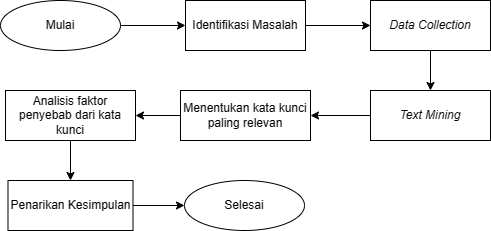
\includegraphics[width=0.825\linewidth]{img/bab3-11.png}
    \caption{Diagram Alir Penelitian}
    \label{fig:3-11}
\end{figure}

Pada tahapan ketika melakukan \textit{data collection} hingga ke hasil interpretasi, dengan menerapkan skema yang pernah digunakan oleh Lai \cite{lai_content_2015} dengan skemanya yaitu "\textit{social media to-concepts}", secara rinci akan dijelaskan di alur tahapannya sebagai berikut:
\newpage

\begin{figure}
    \centering
    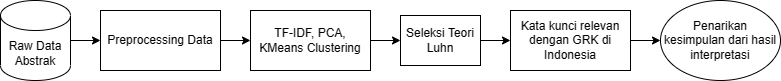
\includegraphics[width=0.95\linewidth]{img/bab3-12.png}
    \caption{Tahapan \textit{Data Collection} hingga hasil interpretasi}
    \label{fig:3-12}
\end{figure}

Berdasarkan tahapan yang digambarkan pada Gambar \ref{fig:3-12}, hal yang pertama dilakukan yaitu identifikasi masalah terkait emisi GRK di Indonesia yang relevan untuk pencarian data yang dilanjutkan dengan studi literatur pada \textit{dataset} yang mendukung untuk mengidentifikasi faktor-faktor penyebab GRK. Adapun pada pemilihan data akan diambil berdasarkan abstrak yang berhubungan dengan GRK di Indonesia, kemudian dilakukan analisis lebih detil terkait relevansi, topik spesifik, dan keterbaruan untuk menentukan teknik apa yang akan digunakan dalam pencarian kata-kata kunci dari \textit{dataset} tersebut.

Selanjutnya, data yang telah dikumpulkan akan diproses menggunakan NLP dengan mengimplementasikan \textit{splitting data} secara Unigram ($\text{N-grams}=1$) untuk mendapatkan kata kunci per huruf dari \textit{dataset}. Kata-kata kunci ini nantinya akan digunakan dalam analisis kualitatif. Dari banyaknya kata kunci tersebut yang memiliki frekuensi paling besar, akan dipilih kata-kata yang paling spesifik berdasarkan teori Luhn. Setelah semua tahapan di atas dilakukan, proses interpretasi akan dilakukan untuk mencari faktor-faktor penyebab GRK berdasarkan hasil yang telah diperoleh. Selanjutnya, akan ditemukan hasil upaya atau solusi dari faktor-faktor penyebab GRK yang telah dipilih berdasarkan kata kunci yang telah didapatkan.

\section{\textit{Data Collection}}
Pada tahapan \textit{data collection}, data yang diambil berdasarkan studi literatur yang telah didapatkan melalui \textit{search engine} Scopus yang mengulas terkait GRK. Data yang diambil tersebut merupakan kumpulan abstrak di artikel atau penelitian yang dipilih berdasarkan pemilihan kata kunci dengan teknik Kitchenham \cite{kitchenham_systematic_2009}. Dalam mendapatkan data studi literatur, diawali dengan mencari faktor-faktor penyebab GRK terlebih dahulu dengan mendapatkan sumber referensi yang telah pernah membahas faktor penyebab GRK. Adapun cara pencariannya terinspirasi dari penelitian yang dilakukan oleh \cite{yunita_finding_2022} dengan melakukan teknik Kitchenham \cite{kitchenham_systematic_2009}.

Pada pencarian studi literatur berupa jurnal atau artikel yang akan dipakai sebagai data penelitian ini, dilakukan pencarian di platform Scopus dengan implementasi Kitchenham yakni mendefinisikan objektif penelitian dengan kata kunci agar didapatkan sekumpulan dan abstrak yang relevan secara efektif. Dimulai dari aspek yang berkaitan dengan penyebab, maka kata kunci yang dipakai yaitu "\textit{factor, feature, variable, cause, character, impact}", kemudian dicari berdasarkan aspek hasil yang ditimbulkan yaitu dengan kata kunci "\textit{affect, contribute, product, generate, conduct}". Setelah itu, dari segi nama subjek yang dipakai mengenai GRK yakni "GHG, \textit{greenhouse gas}", dan yang berdasarkan negara atau daerah spesifik yaitu di Indonesia. Maka, rangkaian kata kunci pencariannya yaitu:
\begin{center}
    \textit{(factor* OR featur* OR variabl* OR caus* OR character* OR impact) AND (affect* OR contribut* OR produc* OR generat* OR conduc*) AND (ghg OR greenhouse AND gas*) AND (indonesia OR indonesian)}
\end{center}

\begin{figure}[!htp]
    \centering
    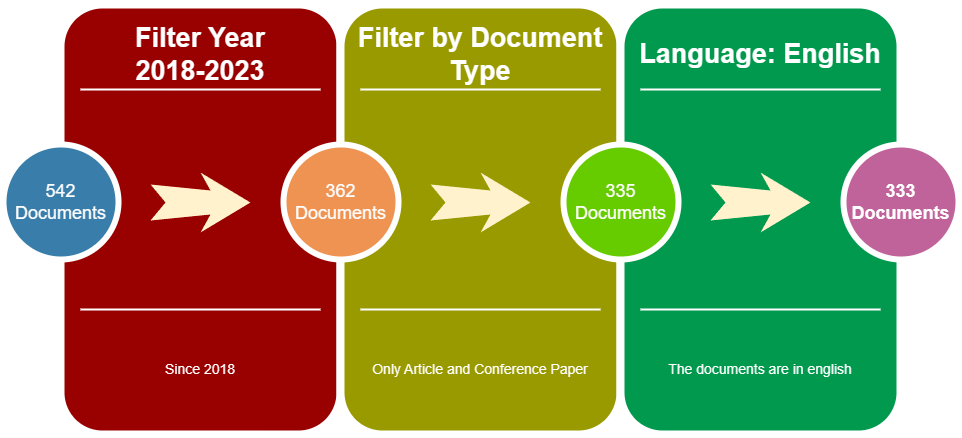
\includegraphics[width=0.85\linewidth]{img/bab3-21.png}
    \caption{Tahapan proses pemilihan data studi literatur}
    \label{fig:3-21}
\end{figure}

Setelah mendefinisikan kata kunci pada pencarian berdasarkan objektif penelitian, terdapat tahapan yang diperlukan dalam pemilihan studi literatur yang cocok sebagaimana yang telah digambarkan pada Gambar \ref{fig:3-21}. Pada pencarian pertama, didapatkan sebanyak 542 dokumen yang tersedia. Agar data studi literatur yang dipakai merupakan dokumen yang baru, maka diambil berdasarkan terbitan publikasi 5 tahun saat ini yaitu tahun 2018 hingga saat ini, maka dihasilkan sebanyak 362 dokumen. Setelah itu, untuk mendapatkan jenis studi literatur yang spesifik, maka dipilih jenisnya yaitu \textit{article} dan \textit{conference paper} dan didapatlah sebanyak 335 dokumen. Pada tahap akhir, dari dokumen studi literatur yang didapat perlu dipilih hanya yang berbahasa Inggris saja, untuk pemahaman dan saat pemrosesan data nanti. 

Berikut ini \textit{query search} yang dihasilkan setelah semua pemilihan dokumen studi literatur tersebut dilakukan di platform Scopus:

\begin{center}
    \textit{TITLE-ABS-KEY ( factor* OR featur* OR variabl* OR caus* OR character* OR impact AND affect* OR contribut* OR produc* OR generat* OR conduc* AND ghg OR greenhouse AND gas* AND indonesia OR indonesian ) AND PUBYEAR $>$ 2017 AND PUBYEAR $<$ 2024 AND ( LIMIT-TO ( LANGUAGE , "English" ) ) AND ( LIMIT-TO ( DOCTYPE , "ar" ) OR LIMIT-TO ( DOCTYPE , "cp" ) )}
\end{center}

Maka, setelah pendefinisian kata kunci dengan teknik Kitchenham, dilanjutkan dengan penyaringan dokumen di platform Scopus, sebanyak 333 dokumen, akan dipakai teks abstrak sebagai \textit{dataset} dalam penelitian ini.

\section{Tahapan \textit{Text Mining} dan Interpretasinya}
\begin{figure}[H]
    \centering
    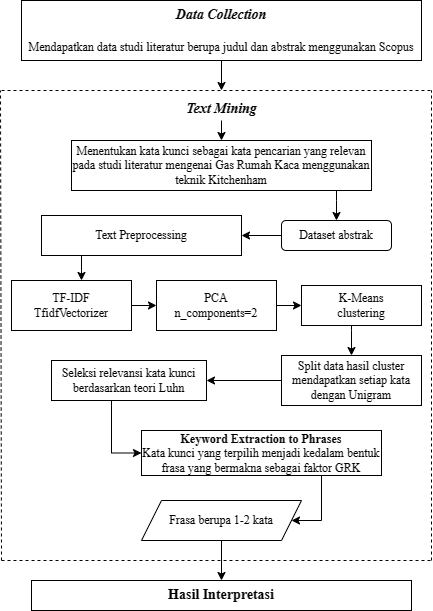
\includegraphics[width=0.7\linewidth]{img/bab3-31.png}
    \caption{Alur tahapan saat dilakukan \textit{text mining} hingga hasil interpretasi}
    \label{fig:3-3}
\end{figure}
Pada tahapan ini, akan lebih banyak implementasi menggunakan NLP, menggunakan data yang berbentuk teks sekumpulan kalimat abstrak yang telah didapatkan, nantinya data tersebut dilakukan \textit{text preprocessing} untuk menyortir teks agar dapat diproses dan siap untuk digunakan dalam analisis lebih lanjut secara baik. Setelah dilakukannya \textit{text preprocessing}, akan dilakukan teknik \textit{clustering} dan dilanjutkan dengan teknik mencari kata kunci yang relevan menggunakan prinsip teori Luhn.

Pada analisis \textit{clustering}, proses tersebut melakukan representasi teks menggunakan TF-IDF, dilanjutkan dengan reduksi dimensi menggunakan PCA, kemudian melakukan K-Means \textit{clustering} untuk mengelompokkan abstrak berdasarkan fitur-fitur yang dihasilkan dari PCA. Hasil akhirnya adalah pengelompokan abstrak ke dalam beberapa klaster berdasarkan kesamaan fitur-fitur TF-IDF yang telah direduksi secara dimensinya menggunakan PCA.

Kemudian pada analisis seleksi kata-kata dasar yang menjadi kata kunci yang memiliki relevansi dengan faktor penyebab GRK, akan diseleksi kata kunci apa 
yang sesuai berdasarkan cara dari teori Luhn. Nantinya dari data berupa kata kunci yang terpilih atau terseleksi tersebut, serta hasil dari \textit{clustering} sebelumnya, akan dipakai di dalam mencari hasil interpretasi berupa faktor dan subfaktor apa yang sering dibahas sebagai penyebab GRK di Indonesia, dan diakhiri dengan penarikan kesimpulan.